\chapter{Extension: Equality Handling and Polynomial Constraint over Integers}

\section{SAT on Equality by Intermediate Value Theorem} \label{sec:eq}
\subsection*{Single Equation}
For solving polynomial constraints with single equality ($g=0$), we apply {\em Intermediate Value Theorem}. 
That is, if existing 2 test cases such that $g > 0$ and $g < 0$, then $g=0$ is SAT somewhere in between. 

\begin{lemma} \label{lemma:ivt}
For $\varphi = \bigwedge \limits_{j}^m f_j > 0~\wedge~g = 0$, $F$ is SAT, if 
there is a box represented by $\Pi = \bigwedge\limits_{v_i \in V}v_i \in (l_i, h_i)$ such that
\begin{enumerate}[(i)]
\item $\bigwedge \limits_{j}^m f_j > 0$ is $\Pi^p_\mathbb{R}$-VALID, and 
\item there are two instances $\vec{t},\vec{t'}$ in the box with $g(\vec{t}) > 0$ and $g(\vec{t'}) < 0$.
\end{enumerate}
\end{lemma}

\begin{proof}
It is clear from the Intermediate Value Theorem that there exist an point $\vec{t_0}$ between $\vec{t}$ and $\vec{t'}$ such that $g(\vec{t_0}) = 0$. In addition, because $\bigwedge \limits_{j}^m f_j > 0$ is $\Pi^p_\mathbb{R}$-VALID, $\vec{t_0}$ also satisfies $\bigwedge \limits_{j}^m f_j > 0$. As a result, $\varphi$ is satisfiable with $\vec{t_0}$ as the SAT instance.
\end{proof}

\begin{example}
Consider the constraint $\varphi = f(x, y) > 0 \wedge g(x, y) = 0$. Suppose we can find a box represented by $\Pi = x \in \langle a, b \rangle \wedge y \in \langle c, d \rangle$ such that $f(x, y) > 0$ is $\Pi^p_\mathbb{R}$-VALID (Figure~\ref{fig:single-equation}). In addition, inside that box, we can find two points $(u_1, v_1)$ and $(u_2, v_2)$ such that $g(u_1, v_1) > 0$ and $g(u_2, v_2) < 0$. By Lemma~\ref{lemma:ivt}, the constraint is satisfiable.
\end{example}
\begin{figure}[ht]
\centering
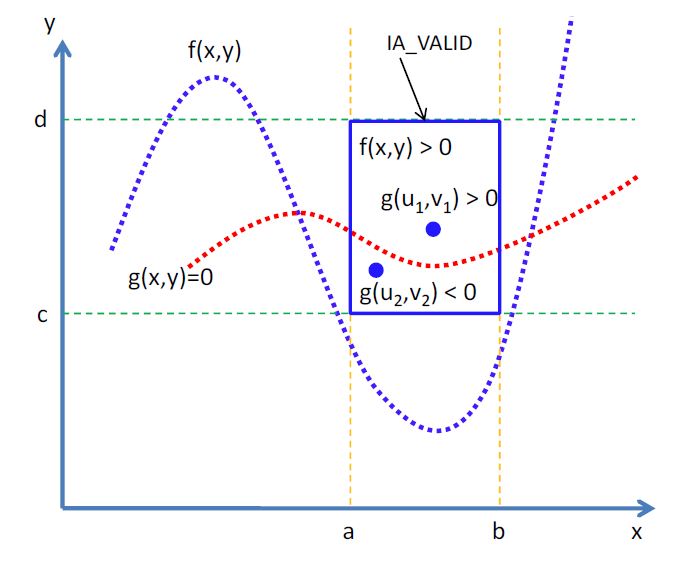
\includegraphics[scale=0.5]{singleEquation.png} 
\caption{Example on solving single equation using the Intermediate Value Theorem} 
\label{fig:single-equation} 
%\end{minipage}
\end{figure} 
{\bf raSAT} first tries to find a box of variables' intervals (by refinements) such that $\bigwedge \limits_{j}^m f_j > 0$ is VALID inside that box. Then it tries to find 2 instances for $g > 0$ and $g < 0$ by testing. 
Intermediate Value Theorem guarantees the existence of an SAT instance in between. 
Note that this method does not find an exact SAT instance. 
\subsection*{Multiple Equations}
The idea of using the Intermediate Value Theorem can also be used for solving multiple equations. Consider $n$ equations ($n \ge 1$): $\bigwedge \limits_{i=1}^n g_i = 0$ and an interval constraint ${\bigwedge\limits_{v_i \in V}v_i \in \langle l_i, h_i \rangle}$. If we can find a set ${\{V_1, \cdots, V_n\}}$ that satisfies the following properties, then we can conclude that $\bigwedge \limits_{i=1}^n g_i = 0$ is satisfiable in ${\bigwedge\limits_{v_i \in V}v_i \in \langle l_i, h_i \rangle}$.
\begin{itemize}
\item For all $i = 1, \cdots, n$; we have ${V_i \subset var(g_i)}$.
\item For all $i \neq j$, we have $V_i \neq V_j$.
\item For all $i = 1, \cdots, n$; let $k_i = |V_i|$ and $V_i = \{v_{ij} \; | \; 1 \le j \le k_i \}$. Then, there exist two values ${(v_{i1}, \cdots, v_{ik_I}) = (x_{i1}, \cdots, x_{ik_i})}$ and ${(v_{i1}, \cdots, v_{ik_I}) = (x'_{i1}, \cdots, x'_{ik_i})}$ such that $g_i(x_{i1}, \cdots, x_{ik_i}, \cdots, v_{ik}, \cdots) * g_i(x'_{i1}, \cdots, x'_{ik_i}, \cdots, v_{ik}, \cdots) < 0$ for all values of $v_{ik}$ in $\langle l_{ik}, h_{ik} \rangle$ where $v_{ik} \in var(g_i) \setminus V_i$.
\end{itemize}
By the first two properties, this method restricts that the number of variables must be greater than or equal to the number of equations.

\begin{example}
Consider two equations $g_1(x, y)=0$ and $g_2(x, y) = 0$ (Figure~\ref{fig:multiple-equations}) which satisfy the above restriction on the number of variables, and the variable intervals is $\Pi = x \in \langle c_1, d_1 \rangle \wedge y \in \langle d_2, c_2 \rangle$. Let $V_1 = \{x\}$ and $V_2 = \{y\}$, we have:
\[g_1(c_1, y)*g_1(d_1, y) < 0 \text{ for all } y \in \langle d_2, c_2 \rangle, \text{ and }\]
\[g_2(x, d_2)*g_2(x, c_2) < 0 \text{ for all } x \in \langle c_1, d_1 \rangle\]
Thus we can conclude that $g_1(x,y)=0 \wedge g_2(x,y=0)$ has a solution inside the box represented by $\Pi$.
\end{example}
\begin{figure}[ht]
\centering
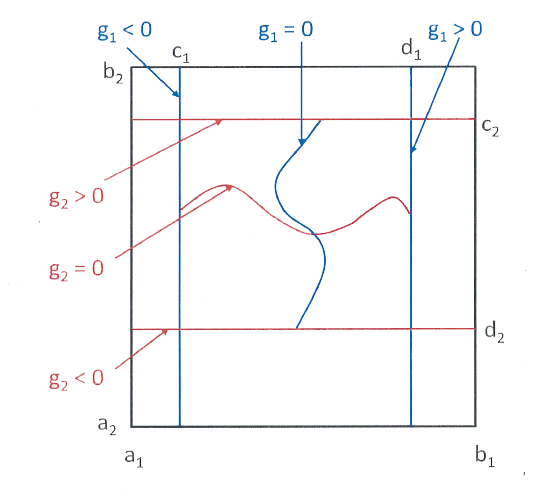
\includegraphics[scale=0.5]{multipleEquations.png} 
\caption{Example on solving single equation using the Intermediate Value Theorem} 
\label{fig:multiple-equations} 
%\end{minipage}
\end{figure}

\section{Polynomial Constraints over Integers} \label{sec:NIA}

{\bf raSAT} loop is easily modified to NIA (nonlinear arithmetic over integers) from NRA, 
by setting $\gamma_0 = 1$ in incremental deepening in Section~\ref{sec:incsearch} 
and restricting tes tdata generation on integers. 
We also compare {\bf raSAT} (combination (1)-(5)-(8)) with {\bf Z3 4.3} on NIA/AProVE benchmark. 
{\bf AProVE} contains 6850 inequalities among 8829. 
Some has several hundred variables, but each API has few variables (mostly just 2 variables). 

The results are, 
\begin{itemize}
\item {\bf raSAT} detects 6764 SAT in 1230.54s, and 0 UNSAT. 
\item {\bf Z3 4.3} detects 6784 SAT in 103.70s, and 36 UNSAT in 36.08s. 
\end{itemize}
where the timeout is $60s$. 
{\bf raSAT} does not successfully detect UNSAT, since UNSAT problems have quite large coefficients
which lead exhaustive search on quite large area. 
%%%%%%%%%%%%%%%%%
\suppress{
\begin{table*}[t]
\centering
\begin{tabular}{ | l | r | r  r | r | r  | r | r | r | r |}
\hline
    \multicolumn{1}{|l|}{Benchmark} & 
    \multicolumn{5}{c|}{\bf raSAT} & \multicolumn{4}{c|}{\bf Z3 4.3)}\\
\hline
    & \multicolumn{3}{|c|}{SAT} & \multicolumn{2}{|c|}{UNSAT} 
    & \multicolumn{2}{|c|}{SAT} & \multicolumn{2}{|c|}{UNSAT} \\
\hline
AProve (6850) & 6764 & 1230.54 & (s) & 0 & 0.00 & 6784 & 103.70 & 36 & 36.08 
\\
\hline
\end{tabular}
\medskip 
\caption{Comparison on NIA/AProVE} \label{tab:aprove}
\end{table*}
}

\subsection*{Experiments on Benchmarks}
In Table \ref{tab:eqexp} we show preliminary experiment for 15 problems that contain polynomial equalities in Zankl family. \textbf{raSAT} works well for these SAT problems and it can detect all SAT problems (11 among 15). At the current implementation, raSAT reports \emph{unknown} for UNSAT problems. The first 4 columns indicate \emph{name of problems}, \emph{the number of variables}, \emph{the number of polynomial equalities} and \emph{the number of inequalities}  in each problem, respectively. The last 2 columns show comparison results of \textbf{Z3 4.3} and \textbf{raSAT}.
\begin{table}
\centering
\scalebox{1.0}{
\begin{tabular}[b]{|c|c|c|c|c|c|c|c|}
\hline
%\multirow{2}{*}{Problem} & {No.} & {No.} & {No.}&
{Problem} & {No.} & {No.} & {No.}&
\multicolumn{2}{c|}{\textbf{Z3 4.3} (15/15)} &\multicolumn{2}{c|}{\textbf{raSAT} (15/15)}\\
\cline{5-8}
Name & Variables& Equalities& Inequalities&{Result} & {Time(s)}&{Result} & {Time(s)}\\
\hline
gen-03 & 1 & 1 & 0& SAT &0.01 & SAT &0.001\\
\hline
gen-04 & 1 & 1 & 0& SAT &0.01 & SAT &0.001\\
\hline
gen-05 & 2 & 2 & 0& SAT &0.01 & SAT &0.003\\
\hline
gen-06 & 2 & 2 & 1& SAT &0.01 & SAT &0.005\\
\hline
gen-07 & 2 & 2 & 0& SAT &0.01 & SAT &0.002\\
\hline
gen-08 & 2 & 2 & 1& SAT &0.01 & SAT &0.009\\
\hline
gen-09 & 2 & 2 & 1& SAT &0.03 & SAT &0.007\\
\hline
gen-10 & 1 & 1 & 0& SAT &0.02 & SAT &0.002\\
\hline
gen-13 & 1 & 1 & 0& UNSAT &0.05 & UNSAT &0.002\\
\hline
gen-14 & 1 & 1 & 0& UNSAT &0.01 & UNSAT &0.002\\
\hline
gen-15 & 2 & 3 & 0& UNSAT &0.01 & UNSAT &0.03\\
\hline
gen-16 & 2 & 2 & 1& SAT &0.01 & SAT &0.006\\
\hline
gen-17 & 2 & 3 & 0& UNSAT &0.01 & UNSAT &0.03\\
\hline
gen-18 & 2 & 2 & 1& SAT &0.01 & SAT &0.002\\
\hline
gen-19 & 2 & 2 & 1& SAT &0.05 & SAT &0.046\\
\hline
\end{tabular}
}
\caption{Experimental results for 15 equality problems of Zankl family}
\label{tab:eqexp}
\end{table}

%%%%%%%%%%%%%%%%%%%%%%%%%%%%%
